\documentclass{beamer}
\mode<presentation>{\usetheme{Madrid}}

\usepackage[utf8]{inputenc}
% Allows including images.
\usepackage{graphicx}
\setcounter{tocdepth}{1}

\title[Linux containers]{Linux containers}

\author{Bruno Barcarol Guimarães}
\institute[]{\textit{bbgstb@gmail.com}}
\date{2015-07-10}

\begin{document}

\begin{frame}
    \titlepage
\end{frame}

\begin{frame}
    \frametitle{Resumo}
    \tableofcontents
\end{frame}

\section{Visão geral}

\subsection{Tecnologias}

\begin{frame}
    \frametitle{Visão geral - Container}
    container != vm != lxc != docker
\end{frame}

\begin{frame}
    \frametitle{Visão geral - Container}
    container != vm != lxc != docker != \textbf{solução de todos os problemas}
\end{frame}

\begin{frame}
    \frametitle{Visão geral - Container}
    Container
    \begin{itemize}
        \item um processo (ou grupo de processos)
        \item executando em um mesmo \textit{kernel} (\textit{i.e.} o kernel
        não é virtualizado)
        \item com diferentes níveis de isolamento entre os outros processos e
        recursos desse \textit{kernel}
    \end{itemize}
\end{frame}

\begin{frame}
    \frametitle{Visão geral - Tecnologias}
    \centering
    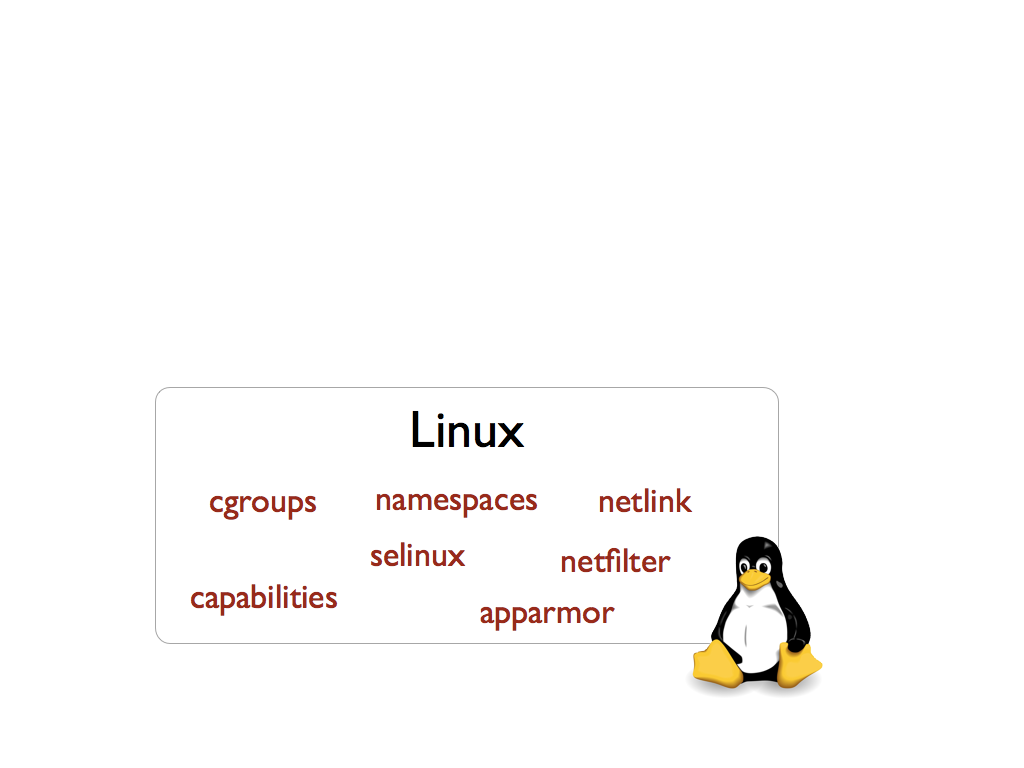
\includegraphics[width=1\linewidth]{img/docker_diagram_kernel.png}
\end{frame}

\begin{frame}
    \frametitle{Visão geral - Tecnologias}
    \centering
    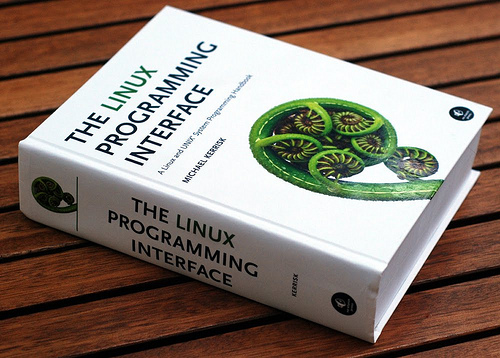
\includegraphics[width=0.8\linewidth]{img/the-linux-programming-interface.jpg}
\end{frame}

\begin{frame}
    \frametitle{Visão geral - Tecnologias}
    \centering
    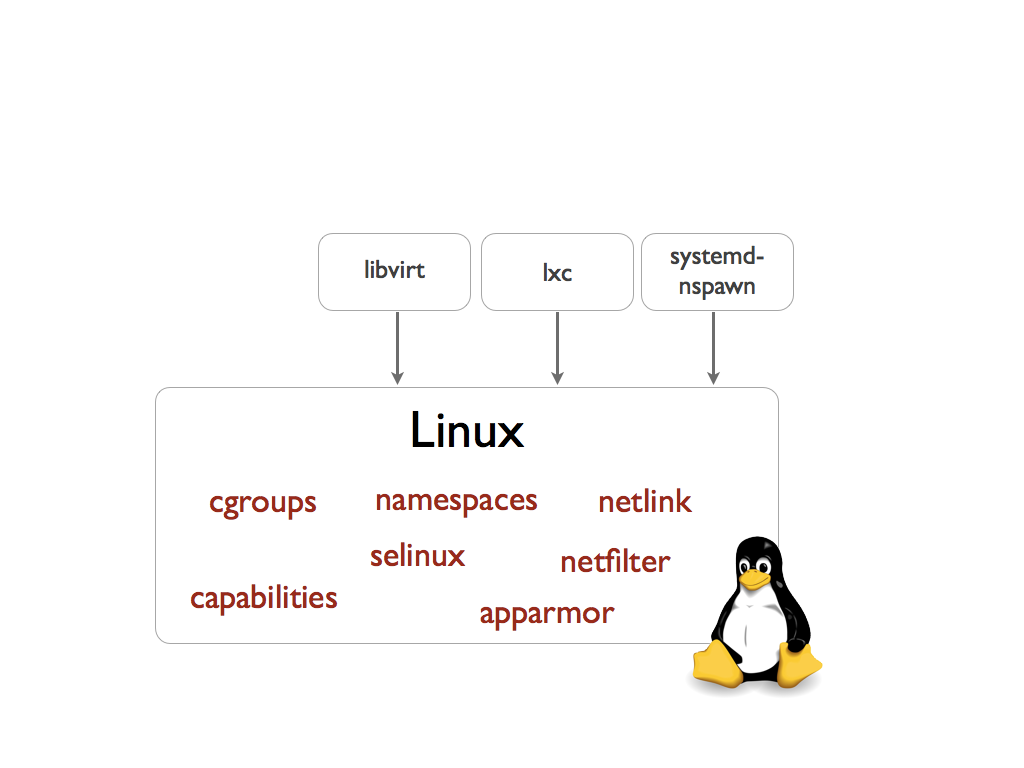
\includegraphics[width=1\linewidth]{img/docker_diagram_lxc.png}
\end{frame}

\begin{frame}
    \frametitle{Visão geral - Tecnologias}
    \centering
    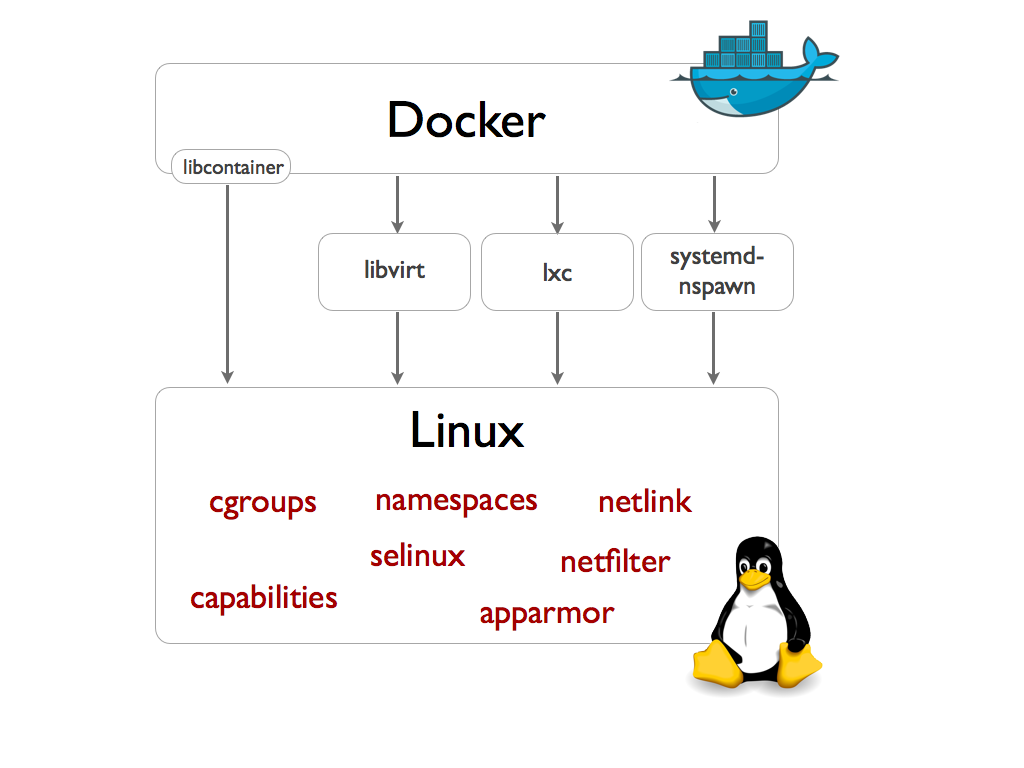
\includegraphics[width=1\linewidth]{img/docker-execdriver-diagram.png}
\end{frame}

\subsection{Vantagens e desvantages}

\begin{frame}
    \frametitle{Visão geral - Vantagens}
    \begin{itemize}
        \item tecnologia nova e em grande expansão
        \item \textit{kernel} compartilhado
            \begin{itemize}
                \item \textit{hardware} não é virtualizado
                \item inicialização mais rápida (\textit{ms})
                \begin{itemize}
                    \item menor \textit{overhead}
                    \item menor utlização de recursos
                \end{itemize}
                \item uma única atualização
                    (\textit{kpatch}/\textit{ksplice}/\textit{live patching}?)
            \end{itemize}
    \end{itemize}
\end{frame}

\begin{frame}
    \frametitle{Visão geral - Desvantagens}
    \begin{itemize}
        \item tecnologia nova e em grande expansão
        \item \textit{kernel} compartilhado
        \begin{itemize}
            \item \textit{hardware} não é virtualizado
            \item apenas um tipo
            \begin{itemize}
                \item versão
                \item arquitetura
                \item sistema operacional
            \end{itemize}
            \item \textit{kernel exploits}
        \end{itemize}
    \end{itemize}
\end{frame}

\begin{frame}
    \frametitle{Visão geral}
    \begin{quote}
        There’s an additional advantage to containerizing your application. It
        forces you to think hard about configuration, limiting the amount of
        mutable state inside your environment and your ability to scale
        horizontally. An exercise in switching to container-based deploys is
        actually an exercise in good engineering practices and any extra work
        required by Docker pays off by making your codebase better factored and
        less brittle. Onwards to excellence, riding the blue container whale!
    \end{quote}
    Jan Urbański - New Relic
\end{frame}

\begin{frame}
    \frametitle{Visão geral}
    \centering
    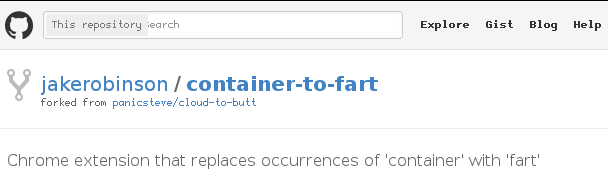
\includegraphics[width=0.8\linewidth]{img/chrome_extension.png}
\end{frame}

\section{Implementação}

\subsection{Kernel}

\begin{frame}
    \frametitle{Implementação - Kernel}
    \begin{itemize}
        \item cgroups
        \item namespaces
    \end{itemize}
\end{frame}

\subsection{cgroups}

\begin{frame}
    \frametitle{cgroups}
    \begin{itemize}
        \item linux 2.6.24 (2007)
        \item limite/reserva de recursos
        \item \textit{accounting}
        \item \textit{audit}
    \end{itemize}
\end{frame}

\subsection{Namespaces}

\begin{frame}
    \frametitle{Namespaces}
    \begin{itemize}
        \item \texttt{clone(2)}
        \item \texttt{unshare(2)}
        \item \texttt{setns(2)}
    \end{itemize}
\end{frame}

\begin{frame}
    \frametitle{Namespaces}
    \begin{itemize}
        \item mnt (\texttt{CLONE\_NEWNS})
        \item uts (\texttt{CLONE\_NEWUTS})
        \item ipc (\texttt{CLONE\_NEWIPC})
        \item pid (\texttt{CLONE\_NEWPID})
        \item net (\texttt{CLONE\_NEWNET})
        \item uid (\texttt{CLONE\_NEWUSER})
    \end{itemize}
\end{frame}

\begin{frame}
    \frametitle{Namespaces - mount}
    \begin{itemize}
        \item \texttt{CLONE\_NEWNS}
        \item linux 2.4.19 (2002)
        \item \texttt{mount(2)/umount(2)}
        \item processos diferentes têm visões diferentes do sistema de arquivos
        \item ``\texttt{chroot(2)} \textit{on steroids}''
        \item compartilhamento de \textit{mount points}
    \end{itemize}
\end{frame}

\begin{frame}
    \frametitle{Namespaces - uts}
    \begin{itemize}
        \item \texttt{CLONE\_NEWUTS}
        \item linux 2.6.19 (2006)
        \item \texttt{uname(2)}/\texttt{sethotname(2)}/\texttt{setdomainname(2)}
    \end{itemize}
\end{frame}

\begin{frame}
    \frametitle{Namespaces - ipc}
    \begin{itemize}
        \item \texttt{CLONE\_NEWIPC}
        \item linux 2.6.19 (2006) / linux 2.6.30 (2009)
        \item \texttt{svipc(7)}/\texttt{mq\_overview(7)}
    \end{itemize}
\end{frame}

\begin{frame}
    \frametitle{Namespaces - pid}
    \begin{itemize}
        \item \texttt{CLONE\_NEWPID}
        \item linux 2.6.24 (2008)
        \item processos em \textit{containers} diferentes podem ter o mesmo pid
        \item processos só vêem outros processos do mesmo \textit{namespace}
        \item migração entre \textit{hosts}
        \item múltiplos pid 1
        \item mapeamento de pid
        \item podem ser aninhados
    \end{itemize}
\end{frame}

\begin{frame}
    \frametitle{Namespaces - net}
    \begin{itemize}
        \item \texttt{CLONE\_NEWNET}
        \item linux 2.6.24 (2008)
        \item cada \textit{namespace} tem seus próprios
            \begin{itemize}
                \item dispositivos de rede
                \item endereços ip
                \item tabelas de roteamento
                \item \texttt{/proc/net}
                \item portas
                \item etc
            \end{itemize}
    \end{itemize}
\end{frame}

\begin{frame}
    \frametitle{Namespaces - user}
    \begin{itemize}
        \item \texttt{CLONE\_NEWUSER}
        \item linux 2.6.23 (2007)
        \item finalizado no kernel 3.8 (2013) $->$ $\sim$ cinco anos
        \item isolamento e mapeamento de uid e gid
        \item \texttt{uid 0}
        \item recursivos
        \begin{itemize}
            \item um processo sem privilégios pode criar um \textit{namespace}
            \item \texttt{uid 0} dentro do \textit{namespace}
            \item ö
        \end{itemize}
    \end{itemize}
\end{frame}

\section{Segurança}

\subsection{uid 0}

\begin{frame}
    \frametitle{Segurança - uid 0}
    \begin{itemize}
        \item não use
    \end{itemize}
\end{frame}

\begin{frame}
    \frametitle{Segurança - uid 0}
    \begin{quote}
        For repos we recognize on or after 2015-01-01, linux builds are sent to
        our container-based infrastructure.
    \end{quote}
    Travis CI
\end{frame}

\begin{frame}
    \frametitle{Segurança - uid 0}
    \begin{quote}
        This job is running on container-based infrastructure, which does not
        allow use of 'sudo', setuid and setguid executables.  If you require
        sudo, add 'sudo: required' to your .travis.yml
    \end{quote}
    Travis CI
\end{frame}

\subsection{Aplicações}

\begin{frame}
    \frametitle{Segurança - Aplicações}
    A maioria dos \textit{containers} executa uma tarefa específica, ao invés
    de um sistema completo, e a maioria dessas aplicações (apache, postgresql,
    mongodb, redis, ...) não precisa de privilégios de root. Os riscos são os
    mesmo que existiram até hoje: assumir que a aplicação pode fazer qualquer
    coisa para escapar do isolamento.
\end{frame}

\begin{frame}
    \frametitle{Segurança - Aplicações}
    syscalls
    \begin{itemize}
        \item e.g. \texttt{vmsplice(2)}
        \item limitar as \textit{syscalls} disponíveis
        \item seccomp/seccomp-bpf
        \item \textit{capabilities}
        \item grsec
        \item atualizações frequentes
    \end{itemize}
    = reduzir a área de exposição do kernel
\end{frame}

\begin{frame}
    \frametitle{Segurança - Aplicações}
    \begin{itemize}
        \item uid \textit{container} $->$ uid diferente no \textit{host}
        \item selinux/apparmor
        \item docker (experimental)
    \end{itemize}
\end{frame}

\begin{frame}
    \frametitle{Segurança - Aplicações}
    \begin{quote}
        ``[...] there's maybe marginal increases in practical security for
        certain kinds of deployment, and perhaps marginal decreases for others.
        We end up coming back to the attack surface, and it seems inevitable
        that that's always going to be larger in container environments. The
        question is, does it matter? If the larger attack surface still only
        results in one more vulnerability per thousand years, you probably
        don't care. The aim isn't to get containers to the same level of
        security as hypervisors, it's to get them close enough that the
        difference doesn't matter.''
    \end{quote}
    Matthew Garrett
\end{frame}

\section{Ferramentas}

\subsection{Demos}

\begin{frame}
    \frametitle{Ferramentas - Demos}
    \begin{itemize}
        \item systemd-nspawn
        \item lxc
        \item docker
    \end{itemize}
\end{frame}

\begin{frame}
    \frametitle{Ferramentas - Futuro}
    \begin{itemize}
        \item Software livre
        \item OCP (\textit{Open Container Project})
        \item FreeBSD docker port
        \item rkt/runc
        \item puppet/ansible ("Glorified Shell Script")
        \item live migration (CRIU)
    \end{itemize}
\end{frame}

\section{Referências}

\begin{frame}
    \frametitle{Referências}
    \begin{itemize}
        \item
            \href
                {https://blog.newrelic.com/2015/06/18/zero-to-docker/}
                {Zero to docker}
        \item
            \href
                {https://www.kernel.org/doc/Documentation/cgroups/}
                {cgroup docs}
        \item
            \href
                {https://lwn.net/Articles/531114/}
                {Namespaces in operation}
        \item
            \href
                {http://mjg59.dreamwidth.org/33170.html}
                {Linux Container Security}
        \item
            \href
                {http://www.slideshare.net/jpetazzo/docker-linux-containers-lxc-and-security}
                {Docker, Linux Containers (LXC), and security}
        \item
            \href
                {https://lwn.net/Articles/268783/}
                {vmsplice(): the making of a local root exploit}
        \item
            \href
                {https://en.wikipedia.org/wiki/Seccomp}
                {seccomp}
        \item
            \href
                {https://en.wikipedia.org/wiki/Grsecurity}
                {grsec}
        \item
            \href
                {http://www.opencontainers.org/}
                {Open Container Project}
        \item
            \href
                {https://github.com/appc/spec/blob/master/SPEC.md}
                {App Container Specification}
    \end{itemize}
\end{frame}

\begin{frame}
    \frametitle{Referências (imagens)}
    \begin{itemize}
        \item http://www.servicioswebgratis.com/wp-content/uploads/2012/08/the-linux-programming-interface.jpg
        \item http://blog.docker.com/2014/03/docker-0-9-introducing-execution-drivers-and-libcontainer/
    \end{itemize}
\end{frame}

\end{document}
